% !TeX encoding = UTF-8
% !TeX spellcheck = pl_PL
\chapter{Tło teoretyczne}

\section{Mikrokontroler}
%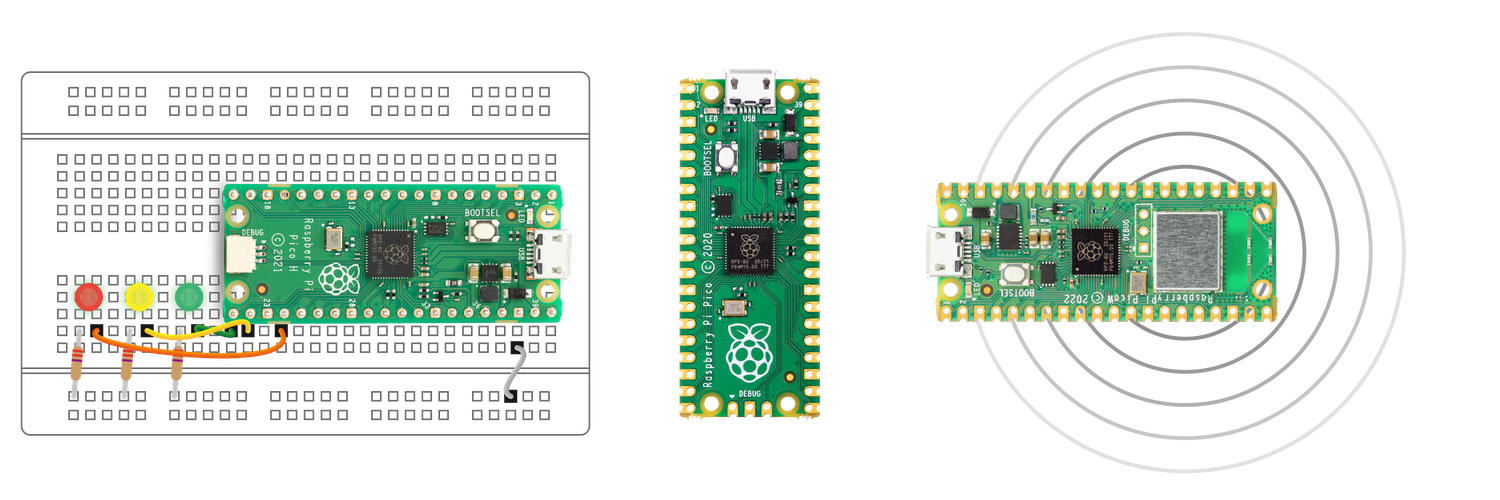
\includegraphics{rp2040.png} // zrobić fotkę mikrokontrolerowy
Mikrokontroler który wykorzystano to Raspberry Pico (RP2040)\cite{pico2024} w rozmiarze (z ang. form factor) 21 mm x 51 mm, z dwu-rdzeniowym procesorem Arm Cortex-M0+, z zegarem o maksymalnym taktowaniu 133 MHz. Ten "mini-komputer" posiada 264 kB SRAM-u i 2 MB pamięci QSPi, 26 wielofunkcyjnych pinów GPIO, włączając w to 3 wejścia analogowe.
Ponadto co jest szczególnie ważne w kwestii przyłączania zewnętrznych modułów mikrokontroler wyposażono w 2 UART, i co mniej ważne 2 SPI, 2 I2C i 16 kanałów PWM.
Do wgrywania programów udostępniono kontroler USB w wersji 1.1, z opcją hosta.
Obsługiwane napięcie wejściowe to od 1,8 V do 5,5 V DC.
Temperatura pracy to od -20 st. C do +85 st. C.
\section{Lora}
Jak podaje artykuł naukowy\cite{Augustin2016} LoRa to bezprzewodowy system telekomunikacyjny o dużym zasięgu, małej mocy i niskiej przepływności, promowany jako rozwiązanie infrastrukturalne dla Internetu rzeczy: urządzenia końcowe wykorzystują LoRa w pojedynczym przeskoku bezprzewodowym, aby komunikować się z bramą (bramkami), podłączonymi do Internetu, które działają jako przezroczyste mosty i przekazują wiadomości między tymi urządzeniami końcowymi a centralnym serwerem sieciowym. W artykule przedstawiono przegląd LoRa i dogłębną analizę jego funkcjonalnych komponentów.
W moim zastosowaniu nie będzie typowych bram, będą po prostu 2 urządzenia działające przy wykorzystaniu tego systemu.
LoRa jest ukierunkowana na zastosowania, w których urządzenia końcowe mają ograniczoną ilość energii (na przykład zasilane z baterii), w których urządzenia końcowe nie muszą przesyłać więcej niż kilka bajtów na raz i w których ruch danych może być inicjowany przez urządzenie końcowe lub przez podmiot zewnętrzny, który chce się z nim skomunikować. Charakter dalekiego zasięgu i niskiego poboru mocy LoRa sprawia, że jest to idealny kandydat do wykorzystania w tym projekcie.
LoRa zapewnia komunikację na duże odległości do 5 km w obszarach miejskich i do 15 km w obszarach wiejskich (w linii wzroku).
Protokół ten umożliwia tworzenie urządzeń, które na zasilaniu bateryjnym mogą działać nawet przez 10 lat.
\section{Bluetooth LE}
Jest to bezprzewodowa sieć osobista (PAN), zaprojektowana i stworzona przez Bluetooth Special Interest Group. Wykorzystuje się ją w opiece zdrowotnej, w branży fitness, w beaconach, bezpieczeństwie i urządzeniach domowej rozrywki. Jest niezależna od klasycznego Bluetooth i nie jest z nim kompatybilna, jednakże te dwie technologie mogą współdziałać w ramach pojedynczego urządzenia.
Sieć ta działa na częstotliwości 2,4 GHz, tak jak klasyczny Bluetooth.
Nominalny zasięg to poniżej 100 m, prędkość od 125 kbit/s do 2 Mbit/s, ilość urządzeń typu slave zależy od implementacji, do zabezpieczenia transmisji wykorzystywany jest 128-bitowy AES.
Sieć ta posiada aktywny frequency hopping, leniwe wiązanie, 24-bitowy klucz CRC i 32-bitowe sprawdzanie integralności wiadomości.
Ze stanu niepołączonego wybudza się w 6 ms, natomiast minimalny czas na wysłanie wiadomości to 3 ms.
Dostępna topologia to z ang. Scatternet.
Moc w zależności od przypadku użycia to 0,01-0,50 W.
Szczytowe natężenie prądu w czasie pracy to mniej niż 15 mA.
Główne zastosowania to telefony mobilne, gaming, inteligentny dom, urządzenia typu wearables, motoryzacja, komputery, bezpieczeństwo, urządzenia zbliżeniowe, ochrona zdrowia, sport, fitness i zastosowania przemysłowe\cite{Wikipedia:ble:2024}.
\section{Micropython}
Jest to podzbiór języka Python 3 przeznaczony do zastosowania w środowiskach o ograniczonych możliwościach pod względem pamięci operacyjnej, mocy procesora czy też maksymalnego zużycia energii elektrycznej. Nie zaimplementowano w nim całego standardu Python 3, jednak jest to dość obszerna implementacja. Nie posiada on własnego środowiska programistycznego (z ang. Integrated Development Environment), zamiast tego zarówno do jego instalacji jak i debugowania stworzonych w nim programów wykorzystuje się aplikację Thonny.
Jest on zoptymalizowany do wykorzystywania na mikrokontrolerach takich jak np. Raspberry Pi Pico, Arduino lub inne.
Kod źródłowy tego oprogramowania dostępny jest na licencji MIT.\cite{wiki:micropython:2024}